\chapter{Background Theory}
The intended outcome of this literature review is to deliver a thorough explanation of the various technologies used throughout the project and to provide details on any additional subject matter aspects which will aid understanding of the project. 

A general summation of Big Data and its application is given in section \ref{bigdata} which is followed by a discussion on the pre-processing of datasets discussed in section \ref{etl}. A high level overview of the NoSQL concept is examined in section \ref{nosql}. The various types of dataset classification which are utilised in the project are given in section \ref{dbclass}.

\section{Big Data}\label{bigdata}
Big Data is a broad, evolving term bound to a complex and powerful application of analytical insight which over recent years has had a variety of definitions. In simplistic terms Big Data can be described as extremely large datasets that may be studied computationally to reveal patterns, trends, and associations for ongoing discovery and analysis.

The 2011 McKinsey Global Institute (MGI), a multinational management consultancy firm, report ``Big data: The next frontier for innovation, competition, and productivity" outlines the potential effects big data will have on a number of industries. The report suggests that with the increasing ``exponential" growth of data volume that simply recruiting a ``few data-orientated managers" will be a temporary fix rather than a lasting solution. MGI suggest that if companies in a variety of sectors such as the healthcare and retail industry were to take advantage of the value which big data brings could see potentially huge returns. ``...a retailer using big data to the full could increase its operating margin by more than 60 percent...healthcare were to use big data creatively and effectively to drive efficiency and quality, the sector could create more than \$300 billion in value every year" \cite{mckinskey}

\subsection{5vs Model}
In 2001, Gartner analyst Doug Laney delivered the original 3vs model which define the challenges and opportunities which have arisen from the increase in data volumes. Laney categorises big data in to three dimensions; Volume, Velocity and Variety, with the increase of each encapsulating the challenges currently faced today of big data management. \begin{figure}[h]\begin{center}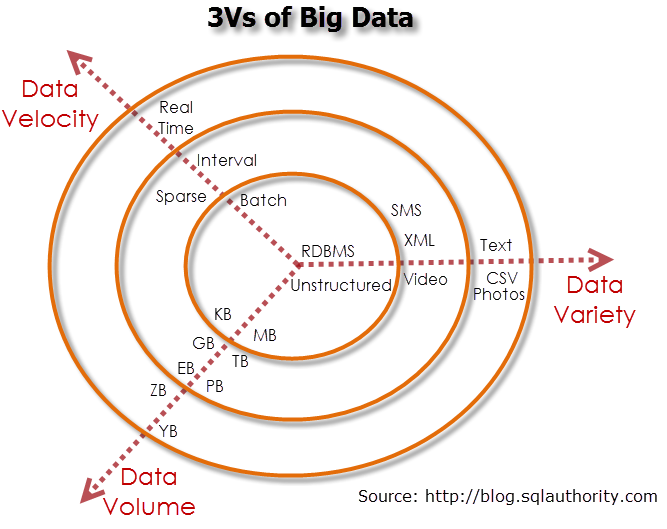
\includegraphics[width=0.8\linewidth]{images/3vs}\caption{3vs data model}\label{fig:3vs}\end{center}\end{figure}The characteristics of each property illustrated in figure \ref{fig:3vs} are defined as: \textbf{Volume} - Refers to the vast amounts of data generated every second. With the creation and storage of large quantities of data, the scale of this data becomes progressively vast. \textbf{Velocity} - Refers to the speed at which new data is generated and the speed at which data moves around emphasising the ``timeliness" of the big data. In order to fully profit from the commercial value of big data, data collection and data examination must be conducted promptly . \textbf{Variety} - This characteristic alludes to the various types of data we can now use; semi-structured and unstructured. Examples being ``audio, video, webpage and text as well as traditional structured data" \cite{bigdata}.

Big Data is a term becoming increasingly common in business and society. Overcoming obstacles and implementing effective, actionable Big Data strategies is key for successful big data management. IBM has introduced a fourth V: \textbf{Veracity} Data inconsistencies and incompleteness result in data uncertainty and unreliability. This creates a new challenge; keeping data organised. \cite{bigdata}

The final and considered by many to be the most important V of big data is \textbf{Value}. ``All the volumes of fast-moving data of different variety and veracity have to be turned into value" \cite{ibm} One of the biggest challenges faced by organisations is having the ability to turn data into something useful.

The amount of data being produced has dramatically increased from when Laney first introduced the 3vs model in 2001. This is in no small part due to the availability and accessibility of the internet. In 1995 the internet had on average 45 million users, 1\% of the worlds population. This figure increased to over 1 billion people with internet access worldwide in 2005, and by 2010 nearly 2 billion which was 30\% of the worlds population. The latest figures show that in 2015 the penetration of the internet reached 3 billion people, 40\% of the entire population. Social media sites such as Facebook, Twitter, Snapchat, Instagram and Pinterest generate millions of  with Facebook boasting 1 million links shared, 2 million friend requests sent and 3 million messages sent on average every twenty minutes \cite{statref}. These statistics show the continual growth of internet accessibility as a whole and with this growth comes the challenge of an amalgamation of the benefit of high volumes of captured analytical data and using this data to add value to an organisation.

\section{Extract Transform Load}\label{etl}
This project will require the extraction, manipulation and processing of a data source from one data model to another. This process is commonly known as Extract Transform Load (ETL). Section \ref{etlprocess} discusses each stage involved in the ETL procedure followed by section \ref{etltool} which examines the ETL implementation methodology and its relevance to this project. 

\subsection{Process}\label{etlprocess}
A basic definition of the Extract Transform Load (ETL) process is pulling data from one database, refactoring the composition of the data and putting the data into another database. While the name ETL implies there are 3 main categorisation stages - extract, transform, load - the procedure in its entirety is a much broader and expansive process which encompass these stages. Despite this the procedure is split in to these three stages. Figure \ref{fig:etl} illustrates the ETL process with data coming from a source; a file or database management system for example then being transformed in to the required format for a successful load. \begin{figure}[h]\begin{center}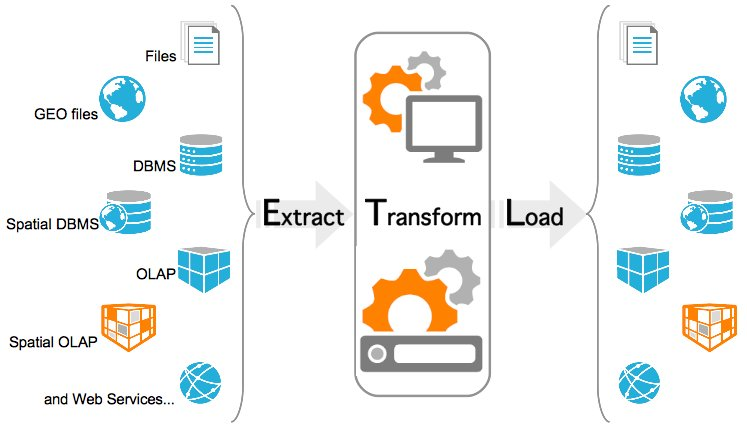
\includegraphics[width=0.8\linewidth]{images/etl.jpg}\caption{ETL process}\label{fig:etl}\end{center}\end{figure}

\textbf{Extract} is the first step in the ETL procedure in which data is read from a source system, usually a database but not restricted to, and makes it available for processing. The main objective of the extract stage is to retrieve all the required data from a source system using as little resources as possible \cite{etlref1}. It is common for data to be extracted from source systems with different organisations and formats to that of the target system. The extract stage provides an opportunity to \textit{cleanse} the data from the source system as often there will be redundant or irrelevant data which is not required.

\textbf{Transform} is where the extracted data is manipulated from its previous state and converted into a target system format. The step involves the application of a set of rules or functions to transform the data from the source to the target. As well as the applied rules and functions the transformation step is responsible for the validation of records ensuring unacceptable records are removed accordingly. ``The most common processes used for transformation are conversion, clearing the duplicates, standardizing, filtering, sorting, translating and looking up or verifying if the data sources are inconsistent." \cite{etlref2}.

\textbf{Load} completes the three step procedure and is where data is written into the target system. There are multiple ways in which data is loaded into a system using the ELT methodology. One of which and the most obvious is to physically insert the data. For example if the target repository is a SQL database insert the data as a new row using the relevant \textit{Insert} statement. An alternative to loading the process manually is that some ETL tool implementations have the capability to ``...link the extraction, transformation, and loading processes for each record from the source." \cite{etlref2}. Depending on the technique applied the load step of the process can become the most time consuming.

\subsection{Tool Implementation}\label{etltool}

Apache Jena (Jena) is a free and open source Java framework for building Semantic Web - discussed in section \ref{semanticweb} - and Linked Data applications. \cite{jena} The Jena framework consists of different APIs interacting together to process Resource Description Framework (RDF) data. I will be using Jena to implement the ETL procedure for the data sources discussed in section \ref{DATA SOURCE REF} as Jena provides an extensive Java library collection for RDF and OWL data representation languages.

W3C defines RDF as ``...a standard model for data interchange on the Web. RDF has features that facilitate data merging even if the underlying schemas differ, and it specifically supports the evolution of schemas over time without requiring all the data consumers to be changed. RDF extends the linking structure of the Web to use URIs to name the relationship between things as well as the two ends of the link (this is usually referred to as a ``triple"). Using this simple model, it allows structured and semi-structured data to be mixed, exposed, and shared across different applications." \cite{rdf}

\section{Knowledge Representation Languages}
A Knowledge Representation (KR) language can be defined as: for any given interpretation of a sentence or string of text the KR must have the ability to effectively and unambiguously express knowledge in a both a human and computer manageable form. 

There are a number of options and possibilities for communicating data and information which range from binary representation to meta markup languages such as Extensible Markup Language (XML) for example. Markup languages which are easily read by humans such as XML which as a result of its rigid set of rules lends its self to both humans and machines. Comparatively binary notation which uses 1's and 0's to represent data, while relatively cheap in terms of computing power the ability to comprehend this notation requires a unique and specific skill set.

\subsection{Semantic Web}\label{semanticweb}
The Semantic Web is an extension of the Web through standards by the World Wide Web Consortium (W3C). ``The standards promote common data formats and exchange protocols on the Web, most fundamentally the Resource Description Framework (RDF)." \cite{semantic}

The Semantic Web has two main intended outcomes. The first is about the standardised formats of data pulled from variety of sources, whereas the original Web concentrated on the interchange of documents \cite{semantic}. The second outcome of the Semantic Web is the language for recording the relation between data and objects in the real world. ``That allows a person, or a machine, to start off in one database, and then move through an unending set of databases which are connected not by wires but by being about the same thing."  \cite{semantic}. 

\subsection{Web Ontology Language OWL}\label{owl}
The Web Ontology Language OWL is a language representation standard for designing and authoring Web ontologies produced from the World Wide Web Consortium W3C. \cite{owl}. The OWL file format is designed to be used by applications required to process the content of the information and to be humanly readable. ``[OWL] is intended to provide a language that can be used to describe the classes and relations between them that are inherent in Web documents and applications."\cite{owl}. The OWL languages are characterised by formal semantics and are built upon the W3C standard RDF format - discussed in section \ref{etltool}

\subsection{OBO}\label{obo}
The OBO flat file format is an ontology representation language. ``The concepts it models represent a subset of the concepts in the OWL description logic language, with several extensions for meta-data modelling and the modelling of concepts that are not supported in DL languages." \cite{obo}

\cite{obo} outlines the intended outcome of the file format aiming to achieve the following criteria :
\begin{itemize}
\item Human readability
\item Ease of parsing
\item Extensibility
\item Minimal redundancy
\end{itemize}

\section{NoSQL}\label{nosql}
NoSQL is labeled as a next generation database known to most as ``Not only SQL" \cite{nosql1}. This definition however insinuates its defiance against the industry standard SQL. It was originally developed in 1998 by Carlo Strozzi; a member of the Italian Linux society, with the intention of being a non-relational, widely distributable and highly scalable database. Strozzi named the database management system NoSQL to merely state it does not express queries in the traditional SQL format. Sadalage and Fowler believe the definition we commonly refer NoSQL as comes from a 2009 conference in San Fransisco held by Johan Oskarsson, a software developer. Sadalage and Fowler recall Oskarssons desire to generate publicity surrounding the event and in an attempt to do so devised the twitter hashtag ``NoSQL Meetup". The main attendees at the conference debrief session were Cassandra, CouchDB, HBase and MongoDB and so the association stuck. \cite{nosql1}

There are are number of key features which encompass the NoSQL framework and encapsulate the essence of its popularity. Many of the NoSQL databases boast their capacity of working in a cluster environment - a cluster being two or more connected computers working collaboratively. Thus delivering a range of options for consistency and distribution  \cite{nosql1}

NoSQL solutions are not bound by a definitive schema structure. This permits the ability to freely adapt database records or add custom fields for example without considering structural changes. This is extremely effective when dealing with varying data types and data sets, in comparison to the traditional relational database model which when tackling this issue often resulted in ambiguous field names.  \cite{nosql1}

\section{Database Classification}\label{dbclass}
One of the first decisions to be made when when selecting a database is the characteristics of the data you are looking to leverage. \cite{nosql2} There are a multitude of options available with many different classifications. The following sections discuss a subset of these which are relevant to this project.

\subsection{Distributed Database}\label{distributeddb}
A distributed database (DDB) comprises of two or more data files located at different sites and servers on a computer network. \cite{dd} The advantage of using a DD is that as the database is distributed, multiple users can access a portion of the database at different locations locally and remotely without obstructing one another's work. It is  pivotal for the DD database management system to periodically synchronise the scattered databases to make sure that they all have consistent data.  \cite{dd} For example if a user updates or deletes data in one location is is essential this change is mirrored on all databases. This ability to remotely access a database from all across the world lends itself to not only multinational companies for example but also startup businesses which recruit the expertise of others from various locations.

\subsection{Document-Oriented Database}
Document-orientated database (DODB) are designed for storing, retrieving and managing document files such as XML, JSON and BSON. The documents stored in a DODB model are data objects which describe the data in the document, as well as the data itself. \begin{figure}[h]\begin{center}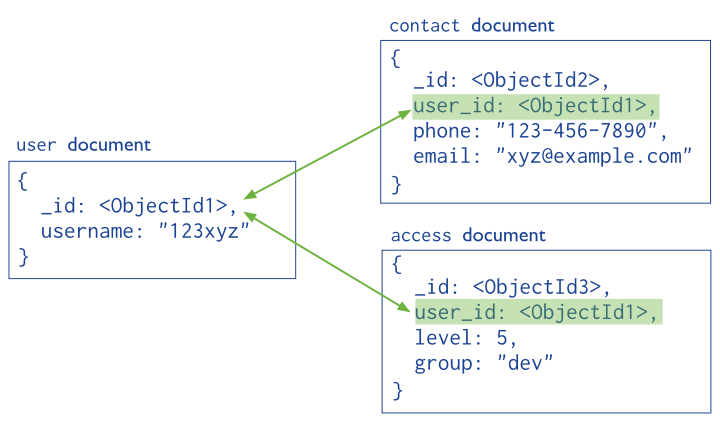
\includegraphics[width=0.75\linewidth]{images/mongodbmodel}\caption{MongoDB document}\label{fig:mongo}\end{center}\end{figure} Figure \ref{fig:mongo} illustrates an example document stored in a DODB specifically in MongoDB. The data is a recognisable JSON format and the joins of the document are between common variable values within each document.

\subsection{Graph-Orientated Database}
A graph-oriented database (GODB), is a form of NoSQL database solution that uses graph theory to store, map and query relationships. A graph is a collection of nodes connected by relationships. ``Graphs represent entities as nodes and the ways in which those entities relate to the world as relationships."  \cite{gd} The formation of the graph database structure is extremely useful and eloquent as it permits clear modelling of a vast and often ecliptic array of data types.  \cite{gd} An example of data represented in a graph structure is the Twitter relationship model. \begin{figure}[h]\begin{center}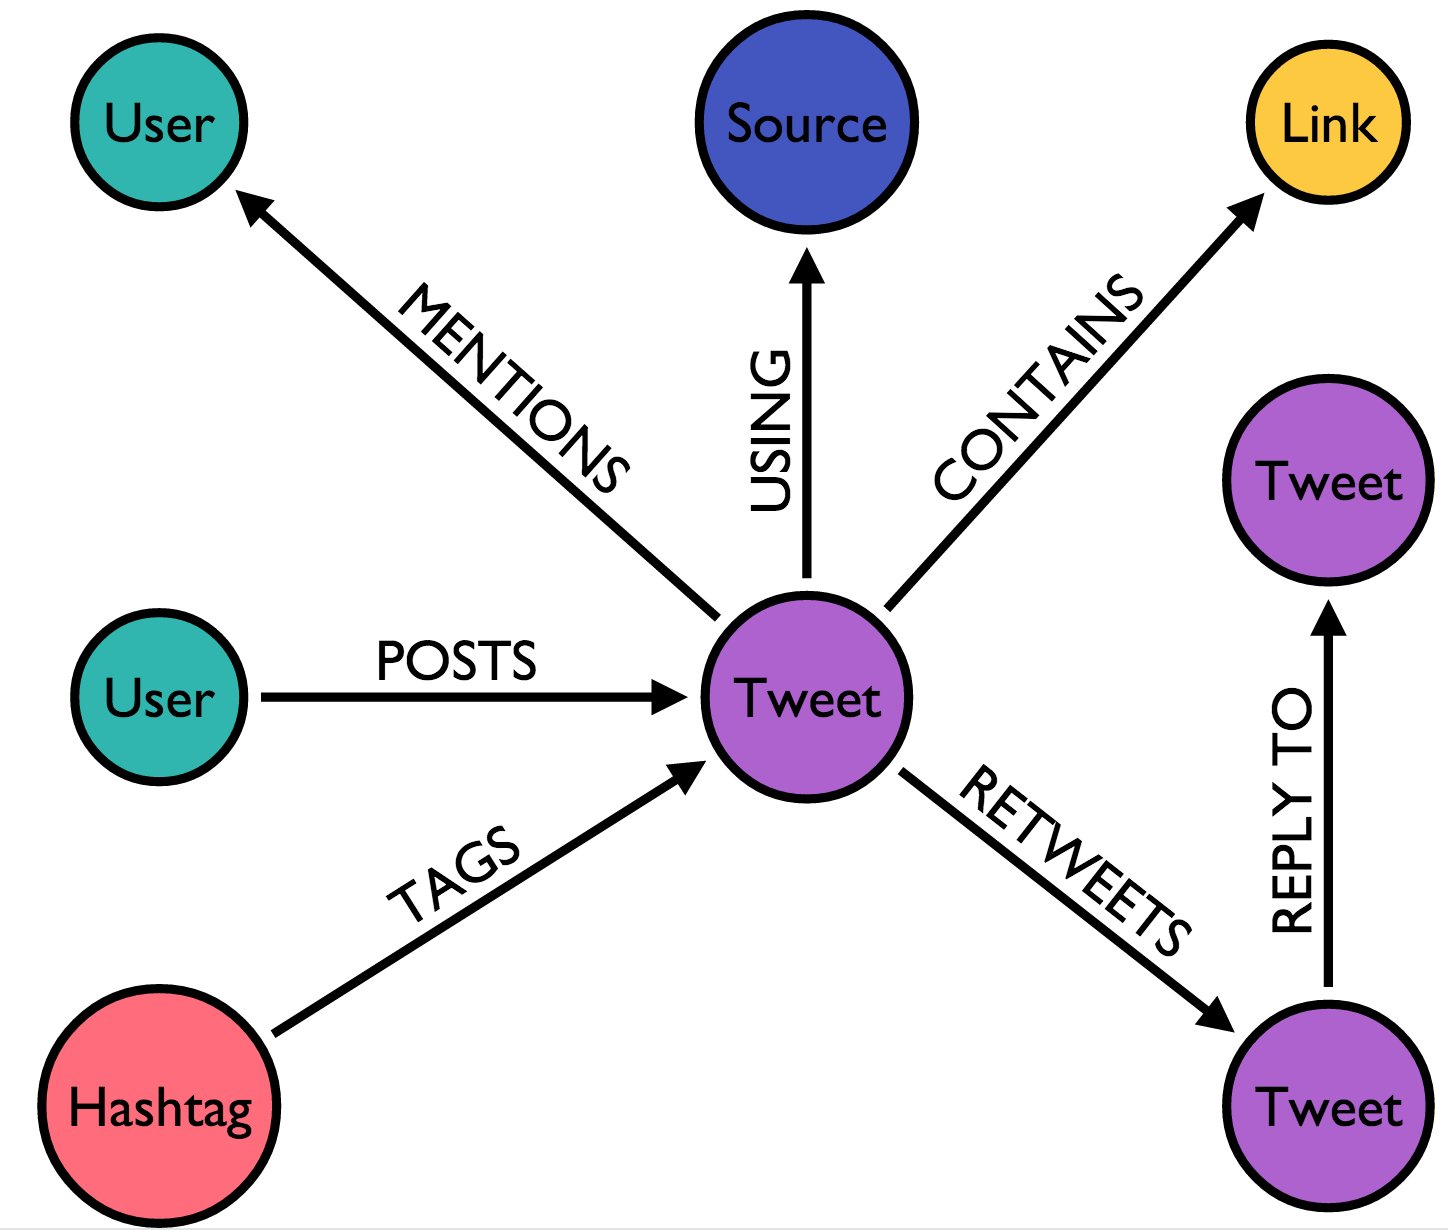
\includegraphics[width=0.5\linewidth]{images/graphdb_twitter}\caption{Example tweet data relationship}\label{fig:twitter}\end{center}\end{figure} Figure \ref{fig:twitter} illustrates the nodes involved in a standard tweet and the relationship link between them. The labeled nodes indicate the various operations which are involved in one the tweet. One interpretation of the figure \ref{fig:twitter} example is that a user posts a tweet, using the Twitter App which mentions another user and includes a hashtag and link.

\subsection{Relational Database}
A relational database (RDB) is a collection of data items organised as a set of tables, records and columns from which data can be accessed or reassembled in many different ways \cite{rdb}. The connected tables are known as relations and contain one or more columns which comprise of data records called rows. Relations can also be instantiated between the data rows to form functional dependencies.

\begin{itemize}
\item One to One: One table record relates to another record in another table.
\item One to Many: One table record relates to many records in another table.
\item Many to One: More than one table record relates to another table record.
\item Many to Many: More than one table record relates to more than one record in another table.
\end{itemize}


\subsection{Column-Orientated Database}
A column-orientated database (CODB) is a database management system that stores data tables as columns of data rather than as rows of data. The main objective of a CODB is to write and read data from the hard disk efficiently in an attempt to speed up querying time. A CODB has the ability to self index which uses less disk space than RDBMS which holds the same data. A CODB can also be highly compressed, resulting in aggregate functions such as MIN, MAX and SUM to be performed at a extremely high rate.  \cite{cd}.

\begin{figure}[h]\begin{center}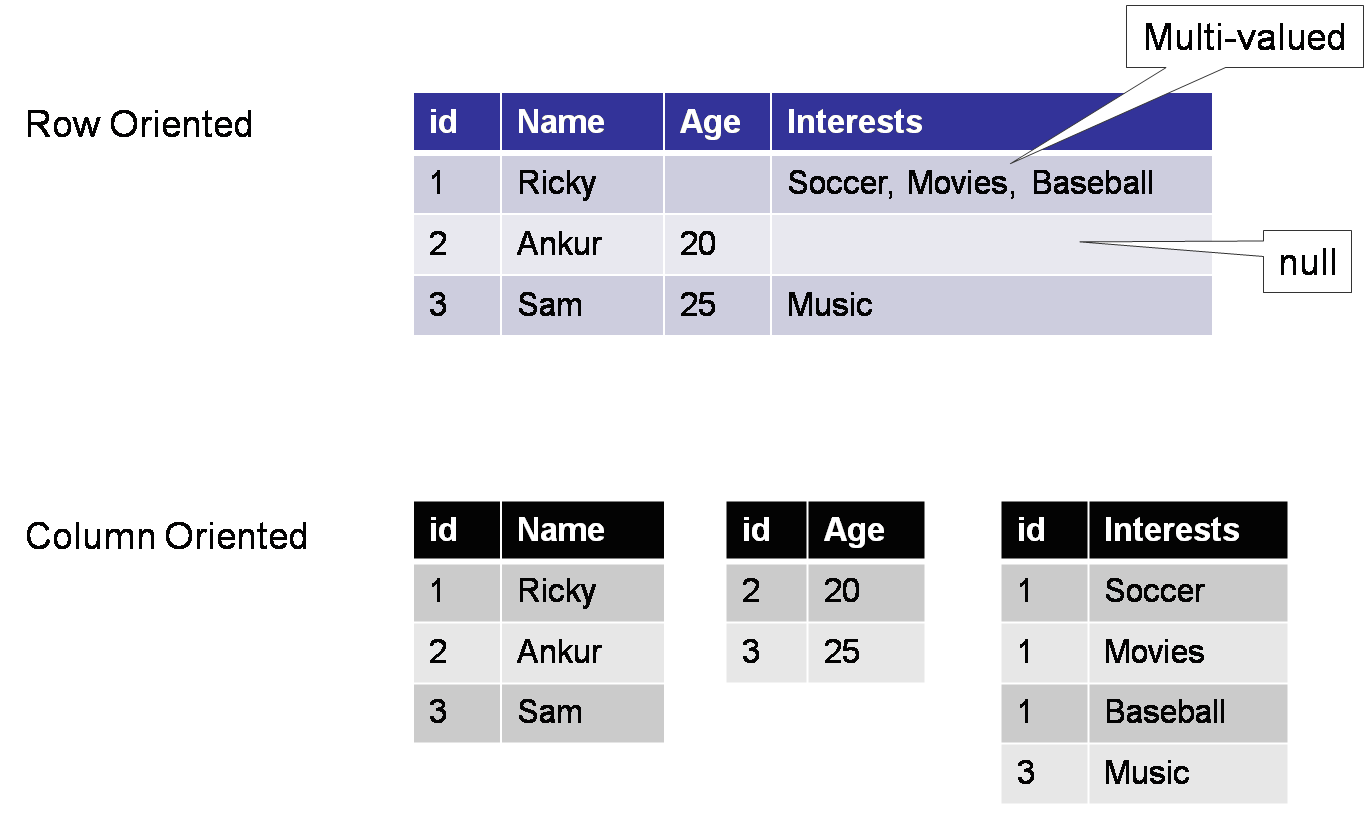
\includegraphics[width=1\linewidth]{images/codb}\caption{Column orientated database example}\label{fig:cod}\end{center}\end{figure}

Figure \ref{cod} illustrates the comparison of a RDB model against a CODB model. Within the row based model the data contains both multiple values per record and null values. However in the CODB model null values are not required as each record contains a minimum and maximum of one value.

\section{Technology Evaluation}\label{techeval}
The technologies being evaluated in this project are outlined below.

\subsection{MongoDB}\label{mongo}
MongoDB is an open source cross-platform DODB. The premise for using MongoDB is simplicity, speed and scalability  \cite{md}. Its ever growing popularity, specifically amongst programmers, stems from the unrestrictive and flexible DODB data model which gives you the ability to query on all fields and boasts instinctive mapping of objects in modern programming languages. \cite{md} The database design of MongoDB is based on the JSON file format named BSON. 

A record in MongoDB is known as a document; a data structure composed of field and value pairs. The values of fields can include other documents, arrays and arrays of other documents. The key features of using MongoDB are its high performance data persistence, provide high availability and automatic scaling  \cite{md}.

\subsection{Neo4j}\label{neo}
Neo4j is an open-source NoSQL GODB which imposes the Property Graph Model throughout its implementation. The team behind the development of Neo4j describe it as an ``An intuitive approach to data problems" \cite{ndweb}. One of the reasons in which Neo4j is favoured predominantly amongst database administrators and developers is its efficiency and high scalability. This is in part due to its compact storage and memory caching for the graphs. ``Neo4j scales up and out, supporting tens of billions of nodes and relationships, and hundreds of thousands of ACID transactions per second." \cite{ndweb}

The key features of Neo4j which lends itself to users, developers and database administrators are its ability to establish relationships on creating, the equality of relationships permits the addition of new relationships being created after initial implementation at no performance cost and its use of memory caching for graphs which allows efficient scaling.

\subsection{Apache Cassandra}\label{cassandra}
Apache Cassandra is an open source column-orientated DDB that is designed for storing and managing vast amounts of data across multiple servers. ``Apache Cassandra is a highly scalable, high-performance distributed database designed to handle large amounts of data across many commodity servers, providing high availability with no single point of failure." \cite{cassandra}. Apache Cassandra define the key features of their database management system as ``continuous availability, linear scale performance, operational simplicity and easy data distribution across multiple data centres and cloud availability zones." \cite{cassandra}.  Figure \ref{fig:cass} illustrates an example record stored in a Cassandra database. \begin{figure}[h]\begin{center}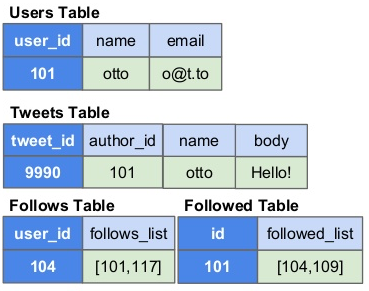
\includegraphics[width=0.70\linewidth]{images/cassandramodel}\caption{Example Cassandra record}\label{fig:cass}\end{center}\end{figure}

\subsection{MySQL}\label{mysql}
MySQL is a freely available open source RDB that uses Structured Query Language (SQL). MySQL is commonly used for web applications with its speed and reliability being a key feature. The MySQL database stores data in tables - a collection of related data - which consists of columns and rows. MySQL runs as a server and allows multiple users to manage and create numerous databases. 

SQL is a programming language used to communicate with databases through queries. SQL queries are used to perform tasks such as update or retrieve data in a database. The queries are in the form of command line language which include keyword statements such as select, insert and update.






